\documentclass[12pt]{article}
\usepackage[T1]{fontenc}
\usepackage[utf8]{inputenc}
\usepackage{polski}
\usepackage{minted}
\usepackage{geometry}
\usepackage{natbib}
\usepackage{enumitem}
\usepackage{graphicx}
\usepackage{bold-extra}
\usepackage[font=small,labelfont=bf]{caption}
\usepackage{hyperref}
\usepackage{titlesec}
\usepackage{indentfirst}
\hyphenpenalty=10000
\tolerance=1000 \emergencystretch=2em
\titlelabel{\thetitle.\quad}

 \geometry{
     left=23mm,
     top=25mm,
     right=23mm
 }


\def\mydate{\leavevmode\hbox{\twodigits\day.\twodigits\month.\the\year}}
\def\twodigits#1{\ifnum#1<10 0\fi\the#1}

\begin{document}
%titlepage
\thispagestyle{empty}
\begin{center}
\begin{minipage}{0.75\linewidth}
    \centering
    
\includegraphics[width=0.45\linewidth]{agh_logo2.png}
    \par
    \vspace{2cm}
    {\bfseries{\scshape{\Huge  Teoria współbieżności}}}
    \par
    \vspace{2cm}
    {\scshape{\Large Laboratorium 5}}
    \par
    \vspace{0.4cm}
    {\scshape{\Large Problem czytelników i pisarzy}}
    \par
    \vspace{3cm}

    {\scshape{\Large Albert Gierlach}}\par
    \vspace{1cm}

    {\Large \mydate}
\end{minipage}
\end{center}
\clearpage



\section{Zadanie 1}
Problem czytelników i pisarzy proszę rozwiązać przy pomocy: semaforów i zmiennych warunkowych

Proszę wykonać pomiary dla różnej ilości czytelników (10-100) i pisarzy (od 1 do 10).
W sprawozdaniu proszę narysować 3D wykres czasu w zależności od liczby wątków i go zinterpretować.

  
\section{Koncept rozwiązania}
Rozwiązanie będzie opierać się na zaimplementowaniu obu metod oraz przeprowadzeniu testów dla różnych konfiguracji. Dla każdej konfiguracji zostanie przeprowadzone 200 iteracji, a wynikiem będzie średni czas działania programu dla zadanych parametrów. Wątek pisarza ma za zadanie wykonać 100 zapisów, a wątek czytelnika 200 odczytów.

Pierwsza metoda będzie opierać się na semaforach (a właściwie mutexach), które będą gwarantować warunki postawione w zadaniu. Uzyte zostaną dwa semafory - jeden dla pisarzy oraz jeden dla czytelników.

Druga metoda opiera się o wykorzystanie zamków (\emph{Lock}) oraz warunków  (\emph{Condition}), które zostaną wykorzystane do prawidłowej synchronizacji między obydwoma typami wątków.

Uśrednione czasy wykonania programu zostaną zapisane do pliku i na ich podstawie zostaną narysowane wykresy. 


\section{Implementacja oraz wyniki}
\begin{minted}[frame=lines,
                framesep=2mm
                ]{java}
interface ILibrary {
    void read() throws InterruptedException;

    void write() throws InterruptedException;
}

class Reader extends Thread {
    private final ILibrary library;
    private final int iters;

    public Reader(ILibrary library, int iters) {
        super();
        this.library = library;
        this.iters = iters;
    }

    @Override
    public void run() {
        for (int i = 0; i < iters; i++) {
            try {
                library.read();
            } catch (InterruptedException exception) {
                break;
            }
        }
    }
}


class Writer extends Thread {
    private final ILibrary library;
    private final int iters;

    public Writer(ILibrary library, int iters) {
        super();
        this.library = library;
        this.iters = iters;
    }

    @Override
    public void run() {
        for (int i = 0; i < iters; i++) {
            try {
                library.write();
            } catch (InterruptedException exception) {
                break;
            }
        }
    }
}

class SemaphoreLibrary implements ILibrary {
    private final Semaphore readerCountSemaphore = new Semaphore(1);
    private final Semaphore writerSemaphore = new Semaphore(1);
    private final AtomicInteger readerCount = new AtomicInteger(0);

    @Override
    public void read() throws InterruptedException {
        readerCountSemaphore.acquire();
        var value = readerCount.incrementAndGet();
        if (value == 1) {
            writerSemaphore.acquire();
        }
        readerCountSemaphore.release();

        // read something

        readerCountSemaphore.acquire();
        value = readerCount.decrementAndGet();
        if (value == 0) {
            writerSemaphore.release();
        }
        readerCountSemaphore.release();
    }

    @Override
    public void write() throws InterruptedException {
        writerSemaphore.acquire();

        // write something

        writerSemaphore.release();
    }
}

class LockLibrary implements ILibrary {
    private final Lock lock = new ReentrantLock();
    private final Condition noWriters = lock.newCondition();
    private final Condition noReadWrite = lock.newCondition();
    private boolean isWriter = false;
    private int readersCount = 0;

    @Override
    public void read() throws InterruptedException {
        lock.lock();
        try {
            while (isWriter) {
                noWriters.await();
            }
            readersCount++;
        } finally {
            lock.unlock();
        }

        // read something

        lock.lock();
        try {
            readersCount--;
            if (readersCount == 0) {
                noReadWrite.signal();
            }
        } finally {
            lock.unlock();
        }
    }

    @Override
    public void write() throws InterruptedException {
        lock.lock();
        try {
            while (readersCount > 0 || isWriter) {
                noReadWrite.await();
            }

            isWriter = true;
        } finally {
            lock.unlock();
        }

        // write something

        lock.lock();
        try {
            isWriter = false;
            noReadWrite.signal();
            noWriters.signal();
        } finally {
            lock.unlock();
        }
    }
}


public class RWMain {

    public static void main(String[] args) {
        var readersNums = List.of(10, 40, 70, 100);
        var writersNums = List.of(1, 4, 7, 10);

        var results = new LinkedList<String>();

        for (var w : writersNums) {
            for (var r : readersNums) {
                ILibrary lib = new SemaphoreLibrary();
                ILibrary lib2 = new LockLibrary();
                var avg1 = testCaseWrapper(r, w, lib);
                var avg2 = testCaseWrapper(r, w, lib2);
                results.add(w + "," + r + "," + round(avg1, 2) + "," + round(avg2, 2));
            }
        }

        Path out = Paths.get("results.csv");
        try {
            Files.write(out, results, Charset.defaultCharset());
        } catch (IOException e) {
            e.printStackTrace();
        }
    }

    public static double round(double v, int places) {
        v = Math.round(v * Math.pow(10, places));
        v = v / Math.pow(10, places);
        return v;
    }

    private static double testCaseWrapper(int r, int w, ILibrary lib) {
        var times = new LinkedList<Long>();

        IntStream.range(0, 200).forEach(i -> {
            long before = System.currentTimeMillis();

            testCase(r, w, lib);

            long diff = System.currentTimeMillis() - before;
            times.add(diff);
        });

        return times.stream().mapToLong(i -> i).average().getAsDouble();
    }

    private static void testCase(int r, int w, ILibrary lib) {
        var executor = Executors.newFixedThreadPool(r + w);
        var threadList = new LinkedList<Thread>();

        IntStream.range(0, r).forEach(i ->
                threadList.add(new Reader(lib, 200))
        );
        IntStream.range(0, w).forEach(i ->
                threadList.add(new Writer(lib, 100))
        );

        threadList.forEach(executor::submit);

        executor.shutdown();
        try {
            executor.awaitTermination(Long.MAX_VALUE, TimeUnit.NANOSECONDS);
        } catch (InterruptedException ignored) {
        }
    }
}
\end{minted}

\noindent
Po wykonaniu programu został stworzony plik results.csv. Wyniki prezentują się następująco:

\begin{center}
\centering
    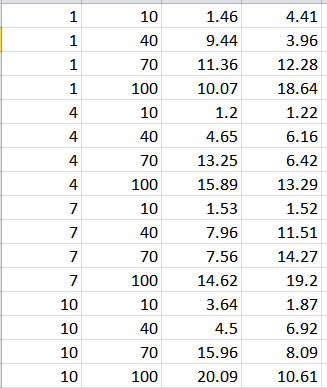
\includegraphics{results.png}
    \captionof{figure}{Wyniki symulacji zapisane w pliku .csv}
\end{center}


\section{Wnioski}
Na podstawie danych został wygenerowan wykres przedstawiający czasy działania programu dla konkretnych konfiguracji. 

\begin{center}
\centering
    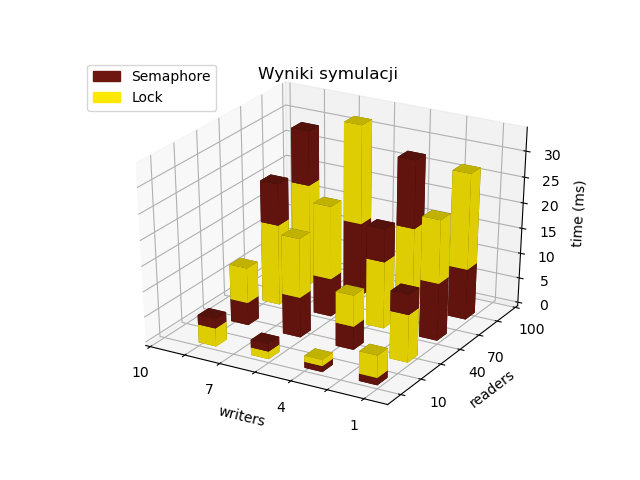
\includegraphics{chart_readers_writers.png}
    \captionof{figure}{Wyniki symulacji}
\end{center}

Powyższy wykres jest wykresem typu \emph{overlapping}, czyli wartości są skumulowane na jednym słupku i nakładają się na siebie. Dzięki temu można szybko zauważyć, która wartość jest większa.

W dziewięciu konfiguracjach szybsze okazały się semafory. Można zauważyć, że w tych konfiguracjach mechanizm zamkowy dodaje spory narzut czasowy. Rozwiązanie z semaforami powoduje, że każdy pisarz musi pozyskać zasób indywidualnie. Oznacza to, że ciąg czytelników może przez pewien czas blokować potencjalnych pisarzy. To rozwiązanie nie jest sprawiedliwe pod względem podziału czasu, ponieważ może dochodzić do zagłodzenia wątków pisarzy.
Drugie rozwiązanie bazujące na zamkach i zmiennych warunkowych jest pół-optymalne. Faworyzuje ono oczekujących pisarzy, więc może dojść do zagłodzenia wątków czytelników. 
Rozwiązanie optymalne może opierać się np. o strukture FIFO, co pozwoliłoby zlikwidować problem zagłodzenia wątków.

\newpage
\section{Zadanie 2}
Proszę zaimplementować listę, w której każdy węzeł składa się z wartości typu Object, referencji do następnego węzła oraz zamka (lock).

Proszę zastosować metodę drobnoziarnistego blokowania do następujących metod listy:
\begin{minted}[frame=lines,
                framesep=2mm
                ]{java}
boolean contains(Object o); //czy lista zawiera element o
boolean remove(Object o); //usuwa pierwsze wystąpienie elementu o
boolean add(Object o); //dodaje element o na koncu listy  
\end{minted}

Proszę porównać wydajność tego rozwiązania w stosunku do listy z jednym zamkiem blokującym dostęp do całości. Należy założyć, że koszt czasowy operacji na elemencie listy (porównanie, wstawianie obiektu) może być duży - proszę wykonać pomiary dla różnych wartości tego kosztu.

\section{Koncept rozwiązania}
Rozwiązanie sprowadza się do implementacji obu typów list oraz zmierzeniu czasów wykonania programu. Zmiennymi parametrami będzie czas wstawiania elementu oraz czas porównania elementu z innym. Każdy test zostanie wykonany 10 razy. Czasy wynikowy będzie średnią z 10 testów. Każdy wątek wykona 30 operacji na liście (dodanie, usunięcie oraz znalezienie elementu). Testy zostaną przeprowadzone dla 2 oraz 8 współdziałających wątków.

\section{Implementacja oraz wyniki}
\begin{minted}[frame=lines,
                framesep=2mm
                ]{java}
public interface ILockedList {
    void add(Object o);

    boolean contains(Object o);

    void remove(Object o);

    void clear();

    int size();
}

class Node {
    private Node next = null;
    private final Lock lock = new ReentrantLock();
    private Object data;

    public Node(Object data) {
        this.data = data;
    }

    public void lock() {
        lock.lock();
    }

    public void unlock() {
        lock.unlock();
    }

    public Node next() {
        return next;
    }

    public void setNext(Node n) {
        next = n;
    }

    public Object getData() {
        return data;
    }
}

public class SingleLockedList implements ILockedList {

    private final Node sentinel = new Node(null);
    private final int insertTime;
    private final int compareTime;
    private final Lock lock = new ReentrantLock();

    public SingleLockedList(int iTime, int cTime) {
        insertTime = iTime * 1000;
        compareTime = cTime * 1000;
    }

    @Override
    public void add(Object o) {
        lock.lock();

        try {
            Node prev = sentinel;
            Node current = sentinel.next();

            while (current != null) {
                prev = current;
                current = current.next();
            }

            try {
                Thread.sleep(0, insertTime);
            } catch (InterruptedException ignored) {
            }

            prev.setNext(new Node(o));
        } finally {
            lock.unlock();
        }
    }

    @Override
    public boolean contains(Object o) {
        lock.lock();
        try {
            Node current = sentinel.next();

            while (current != null) {
                try {
                    Thread.sleep(0, compareTime);
                } catch (InterruptedException ignored) {
                }

                if (current.getData().equals(o)) {
                    return true;
                }

                current = current.next();
            }
        } finally {
            lock.unlock();
        }

        return false;
    }

    @Override
    public void remove(Object o) {
        lock.lock();
        try {
            Node prev = sentinel;
            Node current = sentinel.next();

            while (current != null) {
                try {
                    Thread.sleep(0, compareTime);
                } catch (InterruptedException ignored) {
                }

                if (current.getData().equals(o)) {
                    prev.setNext(current.next());
                    return;
                }

                prev = current;
                current = current.next();
            }
        } finally {
            lock.unlock();
        }
    }

    @Override
    public void clear() {
        sentinel.setNext(null);
    }

    @Override
    public int size() {
        int size = 0;
        Node current = sentinel;
        while(current != null){
            size++;
            current = current.next();
        }

        return size - 1;
    }
}

public class LockedList implements ILockedList {
    private final Node sentinel = new Node(null);
    private final int insertTime;
    private final int compareTime;

    public LockedList(int iTime, int cTime) {
        insertTime = iTime * 1000;
        compareTime = cTime * 1000;
    }

    @Override
    public void add(Object o) {
        Node current = sentinel;
        try {
            current.lock();
            Node next = sentinel.next();

            while (next != null) {
                next.lock();

                Node temp = current;
                current = next;
                temp.unlock();

                next = current.next();
            }

            try {
                Thread.sleep(0, insertTime);
            } catch (InterruptedException ignored) {
            }

            current.setNext(new Node(o));
        } finally {
            current.unlock();
        }
    }

    @Override
    public boolean contains(Object o) {
        Node prev = sentinel;
        Node current = null;
        try {
            prev.lock();
            current = sentinel.next();
            while (current != null) {
                current.lock();

                try {
                    Thread.sleep(0, compareTime);
                } catch (InterruptedException ignored) {
                }

                if (current.getData().equals(o)) {
                    return true;
                }

                prev.unlock();
                prev = current;
                current = current.next();
            }
        } finally {
            if (current != null) {
                current.unlock();
            }
            prev.unlock();
        }
        return false;
    }

    @Override
    public void remove(Object o) {
        Node prev = sentinel;
        Node current = null;
        try {
            prev.lock();
            current = sentinel.next();
            while (current != null) {
                current.lock();

                try {
                    Thread.sleep(0, compareTime);
                } catch (InterruptedException ignored) {
                }

                if (current.getData().equals(o)) {
                    prev.setNext(current.next());
                    return;
                }

                prev.unlock();
                prev = current;
                current = current.next();
            }
        } catch (Exception e){
            e.printStackTrace();
        }
        finally {
            if (current != null) {
                current.unlock();
            }
            prev.unlock();
        }
    }

    @Override
    public void clear() {
        sentinel.setNext(null);
    }

    @Override
    public int size() {
        int size = 0;
        Node current = sentinel;
        while(current != null){
            size++;
            current = current.next();
        }

        return size - 1;
    }
}

class Worker extends Thread {
    private final ILockedList list;
    private final List<Integer> operations;
    private final Random random = new Random();

    public Worker(ILockedList l, List<Integer> op) {
        list = l;
        operations = op;
    }

    @Override
    public void run() {
        for (var op : operations) {
            switch (op) {
                case 0 -> // add
                        list.add(random.nextInt(20));
                case 1 -> // remove
                        list.remove(random.nextInt(20));
                case 2 -> // contains
                        list.contains(random.nextInt(20));
            }

        }
    }
}

public class Main {
    public static void main(String[] args) {
        var insertTime = List.of(10, 500, 999);
        var compareTime = List.of(10, 500, 999);

        var results = new LinkedList<String>();
        for (var i : insertTime) {
            for (var c : compareTime) {
                    var fineGrainedList = new LockedList(i, c);
                    var singleLockedList = new SingleLockedList(i, c);
                    var avg1 = testCaseWrapper(fineGrainedList);
                    var avg2 = testCaseWrapper(singleLockedList);

                    results.add(i + ", " + c + ", "
                        + round(avg1, 2) + ", " + round(avg2, 2));
            }
        }

        Path out = Paths.get("results2.csv");
        try {
            Files.write(out, results, Charset.defaultCharset());
        } catch (IOException e) {
            e.printStackTrace();
        }
    }

    public static double round(double v, int places){
        v = Math.round(v * Math.pow(10, places));
        v = v / Math.pow(10, places);
        return v;
    }

    public static double testCaseWrapper(ILockedList list) {
        var times = new LinkedList<Long>();

        IntStream.range(0, 10).forEach(i -> {
            long before = System.currentTimeMillis();

            testCase(list);

            long diff = System.currentTimeMillis() - before;
            times.add(diff);
        });

        return times.stream().mapToLong(i -> i).average().getAsDouble();
    }

    private static void testCase(ILockedList list) {
        var random = new Random();
        final int OPERATIONS_NUM = 30;
        final int THREAD_NUM = 2;

        var threadList = new LinkedList<Thread>();
        IntStream.range(0, THREAD_NUM).forEach(i -> {
            var op = new LinkedList<Integer>();
            IntStream.range(0, OPERATIONS_NUM).forEach(j -> {
                op.add(random.nextInt(3));
            });
            threadList.add(new Worker(list, op));
        });

        var executor = Executors.newFixedThreadPool(THREAD_NUM);
        threadList.forEach(executor::submit);
        executor.shutdown();

        try {
            executor.awaitTermination(Long.MAX_VALUE, TimeUnit.SECONDS);
        } catch (InterruptedException exception) {
            exception.printStackTrace();
        }

        list.clear();
    }
}
\end{minted}

Wyniki zostały zapisane do plików .csv, a na ich podstawie zostały wygenerowane stosowne wykresy.


\section{Wnioski}
\begin{center}
\centering
    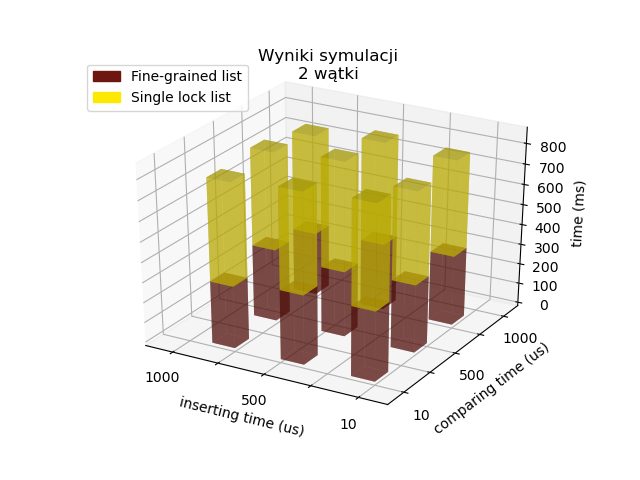
\includegraphics{chart_results_lists_2_threads.png}
    \captionof{figure}{Wyniki symulacji dla dwóch wątków}
\end{center}

\begin{center}
\centering
    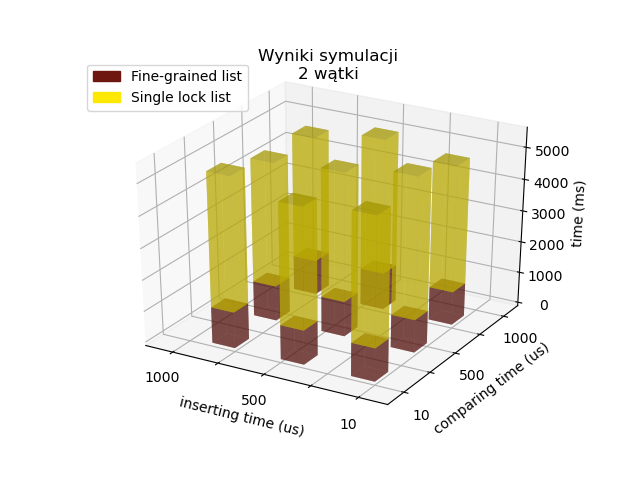
\includegraphics{chart_results_lists_8_threads.png}
    \captionof{figure}{Wyniki symulacji dla ośmiu wątków}
\end{center}


Powyższe wykresy są wykresami typu \emph{overlapping}, czyli wartości są skumulowane na jednym słupku i nakładają się na siebie. Dzięki temu można szybko dostrzec, która wartość jest większa.
Jak można zauważyć - w obu przypadkach szybsza okazała się lista, która stosowała strategię blokowania drobnoziarnistego. Przy dwóch wątkach różnica była na poziomie około 400ms, ale przy ośmiu współbieżnie działających wątkach czasy są znacznie większe.
Powodem takich wyników jest zaleta blokowania drobnoziarnistego, a mianowicie nie blokuje ono całej listy tylko potrzebne węzły, dzięki temu inne wątki mogą operować na części listy. Jednak takie rozwiązanie jest nieoptymalne pod względem pamięciowym, poniważ każdy węzeł musi posiadać blokadę. Podejście to może być bardzo dobrym rozwiązaniem, gdy nasza struktura będzie współdzielona przez wiele wątków, które często będą na niej operować. Dla przypadków, gdzie odwoływanie się do współdzielonej struktury nie będzie zbyt częste, lepszym rozwiązaniem może okazać się struktura, która pozwala na dostęp tylko jednemu wątkowi.

\newpage
\section{Bibliografia}
\begin{itemize}
    \item \url{https://docs.oracle.com/javase/1.5.0/docs/api/java/util/concurrent/locks/Condition.html}
    \item \url{http://home.agh.edu.pl/~funika/tw/lab5/RW-problem.pdf}
    \item \url{https://en.wikipedia.org/wiki/Readers%E2%80%93writers_problem}
    \item \url{https://mieszkomakuch.github.io/problemy-synchronizacyjne/doc/readers-writers.html}
    \item \url{http://www.cs.cmu.edu/afs/cs/academic/class/15418-f18/www/lectures/17_lockfree.pdf}
\end{itemize}

\end{document}
